\section{Convolutions on Manifolds}\label{sec:manifold_cnns}

While group convolutions exploit specific algebraic symmetries, convolutions on manifolds address the fundamental challenge of extending convolutional operations to general geometric spaces. This section examines how the concepts of differential geometry provide the tools necessary to generalize \glspl{CNN} beyond regular grids, preserving the intrinsic geometric structure of the data.

Riemannian manifolds appear naturally in numerous applications: 3D surfaces in computer graphics, configuration spaces in robotics, and high-dimensional data structures in machine learning. The ability to process data directly on these spaces, without resorting to Euclidean approximations that can introduce distortions, represents a significant conceptual advance.

\subsection{Geodesic CNNs}\label{subsec:geodesic_cnns}

Group convolutions provide an elegant framework for extending classical \glspl{CNN} while maintaining specific symmetries such as rotations and translations. However, much real-world data resides in spaces that do not admit a natural group structure, but rather possess a more general geometry characterized by local curvatures and varying metrics. This observation motivates the extension towards \textbf{Riemannian manifolds}, where geodesic CNNs emerge as the first systematic generalization of convolutional operations to non-Euclidean spaces.

\subsubsection{Transition: From Groups to Manifolds}

\paragraph{Limitations of Group Convolutions}

Although group convolutions elegantly capture discrete and continuous symmetries, they face fundamental limitations when the data does not exhibit clear group symmetries:

\begin{enumerate}
    \item \textbf{Variable local geometry}: Data on curved surfaces does not admit globally consistent translations
    \item \textbf{Intrinsic curvature}: The local geometry varies from point to point, invalidating uniform convolution kernels
    \item \textbf{Natural coordinates}: Many domains (surfaces, manifolds) lack canonical global coordinate systems
\end{enumerate}

\begin{example}[Curved Surfaces]
Consider the analysis of 3D shapes represented as triangulated surfaces. While a sphere admits rotations as global symmetries, an arbitrary surface such as a facial model lacks evident symmetries. The local curvature varies dramatically between different regions (convex nose vs. eye sockets), requiring local geometric adaptation.
\end{example}

\begin{example}[Construction of Geodesic Coordinates on Facial Surfaces]
To illustrate the theoretical construction of geodesic coordinates, let us consider the mathematical analysis of a 3D facial model represented as a Riemannian manifold $(M, g)$:

\textbf{Geometric Configuration}:
The facial surface is characterized by:
\begin{itemize}
    \item Genus-0 topology with approximately $10^4$ discrete points
    \item Variable curvature: nose ($K > 0$), eye sockets ($K < 0$), forehead ($K \approx 0$)
    \item Riemannian metric induced by the embedding in $\mathbb{R}^3$
\end{itemize}

\textbf{Mathematical Construction of the Coordinate System}:

\begin{algorithm}[H]
\caption{Rigorous Construction of Geodesic Charts}
\begin{algorithmic}[1]
    \State Given a center point $p \in M$, determine the injectivity radius $r_{\text{inj}}(p)$
    \State Construct an orthonormal basis $\{e_1, e_2\}$ in $T_p M$ using principal curvature directions
    \State Define the exponential map $\exp_p: B_r(0) \subset T_p M \to M$ with $r < r_{\text{inj}}(p)$
    \State For polar coordinates $(\rho, \theta) \in [0,r] \times [0,2\pi)$:
    \State \quad Map via $q = \exp_p(\rho(\cos\theta \, e_1 + \sin\theta \, e_2))$
    \State Correct by the Jacobian factor $J_p(\rho,\theta) = \sqrt{\det g_{\exp_p(\rho e_\theta)}}$
\end{algorithmic}
\end{algorithm}

\textbf{Fundamental Geometric Properties}:
\begin{itemize}
    \item \textbf{Positive curvature (nose)}: $\det(\text{d}\exp_p) < 1$, geodesic concentration
    \item \textbf{Negative curvature (sockets)}: $\det(\text{d}\exp_p) > 1$, geodesic divergence
    \item \textbf{Zero curvature (forehead)}: $\det(\text{d}\exp_p) \approx 1$, local Euclidean behavior
    \item \textbf{Automatic adaptation}: The metric $g$ determines the structure of the geodesic chart
\end{itemize}
\end{example}

\paragraph{Riemannian Manifolds as a Generalization}

A \textbf{Riemannian manifold} $(M, g)$ consists of a smooth manifold $M$ equipped with a Riemannian metric $g$ that defines inner products on each tangent space $T_p M$.

\begin{definition}[Riemannian Manifold]
A Riemannian manifold $(M, g)$ is a differentiable manifold $M$ together with a metric tensor $g$ that assigns to each point $p \in M$ an inner product $g_p: T_p M \times T_p M \to \mathbb{R}$ that varies smoothly with $p$.
\end{definition}

This structure allows defining fundamental geometric concepts:
\begin{itemize}
    \item \textbf{Geodesic distances}: $d_g(p,q) = \inf_{\gamma} \int_0^1 \sqrt{g_{\gamma(t)}(\dot{\gamma}(t), \dot{\gamma}(t))} dt$
    \item \textbf{Geodesic neighborhoods}: Regions locally isometric to Euclidean spaces
    \item \textbf{Parallel transport}: Mechanism for comparing vectors at different points
\end{itemize}

\subsubsection{Fundamental Architecture: Geodesic CNN}

The seminal work of \citet{masci2018geodesicconvolutionalneural} introduces \textbf{Geodesic CNNs} as the first rigorous extension of convolutional operations to general Riemannian manifolds.

\paragraph{Central Principle: Geodesic Coordinate Systems}

The fundamental idea consists of establishing local coordinate systems around each point of the manifold using \textbf{geodesic coordinates}.

\begin{definition}[Geodesic Coordinates]
Given a point $p \in M$ on a Riemannian manifold, the geodesic coordinates in a neighborhood $U_p$ are defined via the exponential map:
\begin{equation}
\exp_p: T_p M \supset B_\epsilon(0) \to U_p \subset M
\end{equation}
where $B_\epsilon(0)$ is a ball of radius $\epsilon$ in the tangent space $T_p M$.
\end{definition}

\paragraph{Construction of the Geodesic Chart}

For each point $p \in M$, a \textbf{geodesic chart} is constructed that allows defining local convolutional operations:

\begin{algorithm}[H]
\caption{Construction of a Geodesic Chart}
\begin{algorithmic}[1]
    \State \textbf{Input:} Point $p \in M$, geodesic radius $r > 0$
    \State Compute orthonormal basis $\{e_1, e_2\}$ in $T_p M$
    \State Define polar grid: $\{(r_i \cos \theta_j, r_i \sin \theta_j)\}$ in $T_p M$
    \State Map via $\exp_p$ to points $\{q_{ij}\}$ in $M$
    \State Interpolate feature values at the mapped points
    \State \textbf{Output:} Regular geodesic patch around $p$
\end{algorithmic}
\end{algorithm}

\begin{figure}[htbp]
	\centering
	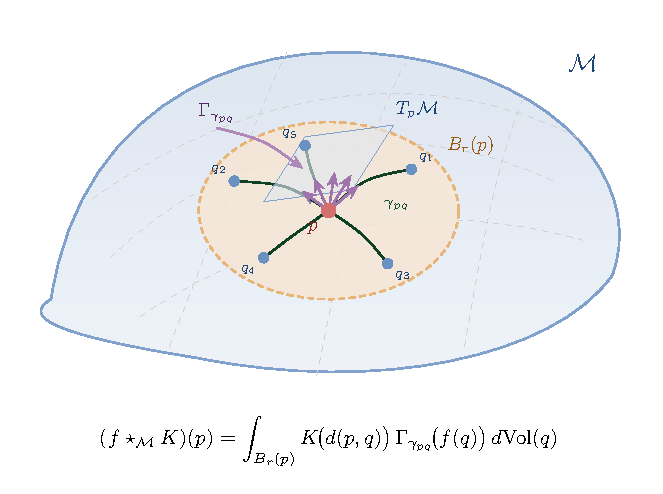
\includegraphics[width=0.80\textwidth]{images/geodesic_convolution}
	\caption[Geodesic convolution on a surface]{Geodesic convolution: the kernel is applied on the geodesic ball $B_r(p)$ around a point $p$ on the surface $\mathcal{M}$, parallel-transporting the features of the neighbors $q_j$ to the tangent space $T_p\mathcal{M}$.}
	\label{fig:geodesic_convolution}
\end{figure}

\paragraph{Geodesic Convolution Operation}

The convolution at point $p$ is defined as:

\begin{equation}
(f * k)_g(p) = \sum_{i,j} k_{ij} \cdot f(\exp_p(r_i e_{\theta_j})) \cdot J_p(r_i, \theta_j)
\label{eq:geodesic_convolution}
\end{equation}

where:
\begin{itemize}
    \item $k_{ij}$ are the learnable kernel weights
    \item $f$ is the feature function on the manifold
    \item $J_p(r_i, \theta_j)$ is the Jacobian correction factor
    \item $e_{\theta_j} = \cos\theta_j e_1 + \sin\theta_j e_2$ are angular directions
\end{itemize}

\subsubsection{Critical Technical Aspects}

\paragraph{Jacobian Correction}

The Riemannian metric introduces distortions that must be compensated. The Jacobian factor corrects the non-uniformity of the exponential map:

\begin{equation}
J_p(r, \theta) = \sqrt{\det g_{\exp_p(r e_\theta)}(\partial_r \exp_p, \partial_\theta \exp_p)}
\end{equation}

\paragraph{Choice of the Tangent Basis}

The construction requires selecting an orthonormal basis in each tangent space $T_p M$. The options include:
\begin{enumerate}
    \item \textbf{Principal directions}: Use eigenvectors of the curvature operator
    \item \textbf{Local consistency}: Minimize variation with respect to neighboring points
    \item \textbf{Parallel transport}: Propagate the basis from a reference point
\end{enumerate}

\subsubsection{Anisotropic Diffusion Descriptors}

Complementing geodesic CNNs, \citet{Boscaini2016AnisotropicDD} introduce \textbf{Anisotropic Diffusion Descriptors} (ADs) that overcome the limitations of isotropic spectral methods.

\paragraph{Motivation: Isotropic Limitations}

Classical spectral descriptors such as Heat Kernel Signatures (HKS) assume isotropic diffusion, losing crucial directional information in shapes with elongated structures or prominent directional features.

\paragraph{Mathematical Formulation}

ADs use an anisotropic diffusion operator parameterized by a conductivity tensor $C_p$:

\begin{equation}
\frac{\partial u}{\partial t} = -\text{div}(C \cdot \nabla u)
\end{equation}

where $C_p$ adapts the diffusion to the local geometry. The solution $u_t(p)$ for different times $t$ and directions generates the descriptor:

\begin{equation}
\text{AD}_p = \{u_t(p, \theta_k) : t \in T, \theta_k \in \Theta\}
\end{equation}

\paragraph{Computational Advantages}

\begin{enumerate}
    \item \textbf{Directional sensitivity}: Captures local orientations of geometric features
    \item \textbf{Robustness}: Stability under isometric deformations
    \item \textbf{Efficiency}: Computation via optimized spectral formulation
\end{enumerate}

\subsubsection{Implementation and Practical Considerations}

\paragraph{Discretization on Triangular Meshes}

In practice, manifolds are represented as triangular meshes. The implementation requires:

\begin{algorithm}[H]
\caption{Geodesic CNN on a Triangular Mesh}
\begin{algorithmic}[1]
    \State Compute the discrete Laplace-Beltrami operator $L$
    \State For each vertex $v_i$:
    \State \quad Estimate the local metric via triangle areas
    \State \quad Construct an orthonormal basis in the discrete tangent space
    \State \quad Compute approximate geodesic distances
    \State \quad Apply bilinear interpolation for regular sampling
    \State Propagate gradients respecting the discrete geometry
\end{algorithmic}
\end{algorithm}

\paragraph{Numerical Stability}

Critical aspects for robust implementations:
\begin{itemize}
    \item \textbf{Adaptive radius}: Adjust $r$ according to local curvature to avoid singularities
    \item \textbf{Geodesic regularization}: Smooth distortions in regions of high curvature
    \item \textbf{Boundary handling}: Special treatment of boundary conditions
\end{itemize}

\subsubsection{Limitations and Motivation for Extensions}

Geodesic CNNs, although revolutionary, present limitations that motivate later developments:

\paragraph{Dependence on Local Coordinates}
The construction of geodesic charts introduces dependencies on the choice of tangent bases, creating potential inconsistency between adjacent regions.

\paragraph{Computational Scalability}
The computation of geodesic coordinates and Jacobian corrections is computationally intensive, especially for high-resolution manifolds.

\paragraph{Limitation to Smooth Geometries}
The exponential map requires sufficient differentiability, limiting applicability to manifolds with singularities or discontinuities.

\paragraph{Lack of Globality}
By processing local patches independently, important global geometric correlations are potentially lost.

\textbf{Transition towards General Methods.} These limitations motivate the development of more general approaches that:
\begin{enumerate}
    \item Avoid explicit dependence on coordinate systems
    \item Incorporate global information efficiently
    \item Handle manifolds with complex or discontinuous geometries
    \item Provide theoretical guarantees of intrinsic equivariance
\end{enumerate}
This motivation sets the context for the methods that will be developed in the following subsections.

\subsection{General Methods: MoNet}\label{subsec:monet}

MoNet~\citep{DBLP:journals/corr/MontiBMRSB16} introduces a unifying framework that abstracts geometric relationships via \textbf{pseudo-local coordinates}, providing greater flexibility than approaches specific to each type of manifold.

\subsubsection{Theoretical Framework}

\begin{definition}[Pseudo-local Coordinates]\label{def:coordenadas_pseudo_locales}
Pseudo-local coordinates are functions $u: M \times M \to \mathbb{R}^d$ that encode local geometric relationships between pairs of points $(x, y) \in M \times M$, satisfying:
\begin{enumerate}
    \item \textbf{Locality}: $u(x, y) = 0$ if $x$ and $y$ are not in the same local neighborhood
    \item \textbf{Invariance}: $u$ is invariant under isometries of the manifold
    \item \textbf{Differentiability}: $u$ is smooth in the interior of its domain
\end{enumerate}
\end{definition}

\textbf{Fundamental examples of pseudo-local coordinates}:

\begin{enumerate}
    \item \textbf{Geodesic distance and angle}:
    \begin{equation}
    u_{\text{geod}}(x, y) = (d_g(x, y), \angle(x, y))
    \end{equation}
    where $\angle(x, y)$ is the polar angle in geodesic coordinates centered at $x$.

    \item \textbf{Local spectral coordinates}:
    \begin{equation}
    u_{\text{spec}}(x, y) = (\phi_1(x) - \phi_1(y), \phi_2(x) - \phi_2(y), \ldots, \phi_k(x) - \phi_k(y))
    \end{equation}
    using eigenfunctions of the Laplace-Beltrami operator.

    \item \textbf{Heat kernel encoding}:
    \begin{equation}
    u_{\text{heat}}(x, y) = (H_t(x, y))_{t \in T}
    \end{equation}
    where $H_t(x, y) = \sum_{i=0}^{\infty} e^{-\lambda_i t} \phi_i(x) \phi_i(y)$ is the heat kernel.
\end{enumerate}

\begin{definition}[Generalized MoNet Kernel]\label{def:kernel_monet}
MoNet kernels are defined as linear combinations of parametric basis functions:
\begin{equation}
w_\theta(u) = \sum_{j=1}^J w_j(\theta) \psi_j(u)
\end{equation}
where:
\begin{itemize}
    \item $w_j(\theta)$ are learnable weights dependent on parameters $\theta$
    \item $\psi_j(u)$ are basis functions (typically Gaussian)
    \item $u$ are pseudo-local coordinates
\end{itemize}

For the specific case of Gaussian mixtures:
\begin{equation}
w_\theta(u) = \sum_{j=1}^J \alpha_j(\theta) \exp\left(-\frac{1}{2}(u - \mu_j(\theta))^T \Sigma_j^{-1}(\theta) (u - \mu_j(\theta))\right)
\end{equation}
\end{definition}

\begin{theorem}[Universal Approximation of MoNet Kernels]\label{thm:universal_approximation_monet}
For any continuous function $k: \mathbb{R}^d \to \mathbb{R}$ with compact support, and for any $\epsilon > 0$, there exists a finite number $J$ and parameters $\{\alpha_j, \mu_j, \Sigma_j\}_{j=1}^J$ such that:
\begin{equation}
\sup_{u \in \text{supp}(k)} |k(u) - w_\theta(u)| < \epsilon
\end{equation}
\end{theorem}

\begin{proof}[Proof sketch]
The proof follows from the density of Gaussian mixtures in $L^2(\mathbb{R}^d)$ and the compactness of the support. The technical details involve:
\begin{enumerate}
    \item Approximation in $L^2$ norm by the Weierstrass approximation theorem
    \item Uniform convergence on compact sets
    \item Control of the approximation error via the number of Gaussian components
\end{enumerate}
\end{proof}

\textbf{MoNet convolution operation}: The convolution at a point $x \in M$ is defined as:
\begin{equation}
(f * w)(x) = \int_{\mathcal{N}(x)} w_\theta(u(x, y)) f(y) dV_g(y)
\end{equation}
where:
\begin{itemize}
    \item $\mathcal{N}(x)$ is a local neighborhood of $x$
    \item $dV_g$ is the Riemannian volume element
    \item $u(x, y)$ are the pseudo-local coordinates
\end{itemize}

\textbf{Discretization on meshes}: For discrete manifolds represented as meshes:
\begin{equation}
(f * w)(x_i) = \sum_{j \in \mathcal{N}(i)} w_\theta(u(x_i, x_j)) f(x_j) A_j
\end{equation}
where $A_j$ are local area weights (e.g., Voronoi areas).

\subsubsection{Unification of Architectures}

MoNet unifies multiple existing architectures via specific choices of coordinates:

\begin{itemize}
    \item \textbf{Geodesic CNNs}: $u(p,q) = (\rho(p,q), \theta(p,q))$
    \item \textbf{Graph CNNs}: $u(p,q) = (\frac{1}{\sqrt{d_p}}, \frac{1}{\sqrt{d_q}})$
    \item \textbf{SplineCNNs}: Coordinates based on B-splines
\end{itemize}

This unification allows transferring intuitions and techniques between different geometric domains.

\begin{example}[Unified Theoretical Framework of MoNet]

To illustrate the versatility of the MoNet framework, we analyze the mathematical formulation of adaptive kernels for three distinct geometric domains:

\textbf{General Mathematical Formulation}:

Let $u: M \times M \to \mathbb{R}^d$ be a pseudo-local coordinate function. MoNet kernels are defined as Gaussian mixtures in the coordinate space:

\begin{equation}
w_\theta(u) = \sum_{j=1}^J \alpha_j \exp\left(-\frac{1}{2}(u - \mu_j)^T \Sigma_j^{-1} (u - \mu_j)\right)
\end{equation}

where $\theta = \{\alpha_j, \mu_j, \Sigma_j\}_{j=1}^J$ are learnable parameters.

\textbf{Specializations by Geometric Domain}:

\begin{enumerate}
    \item \textbf{Riemannian Surfaces}:
    \begin{equation}
    u_{\text{geo}}(p,q) = (\rho_g(p,q), \theta_p(q))
    \end{equation}
    where $\rho_g$ is the geodesic distance and $\theta_p(q)$ is the angle in geodesic polar coordinates centered at $p$.

    \item \textbf{Discrete Graphs}:
    \begin{equation}
    u_{\text{graph}}(i,j) = \left(\frac{1}{\sqrt{d_i}}, \frac{1}{\sqrt{d_j}}\right)
    \end{equation}
    where $d_i, d_j$ are the degrees of vertices $i, j$.

    \item \textbf{Euclidean Grids}:
    \begin{equation}
    u_{\text{grid}}(p,q) = q - p
    \end{equation}
    representing relative Cartesian differences.
\end{enumerate}

\textbf{Unifying Properties of the Framework}:
\begin{enumerate}
    \item \textbf{Mathematical consistency}: All domains reduce to the same Gaussian kernel formulation
    \item \textbf{Theoretical transferability}: The parameters $\theta$ can be transferred between domains with compatible dimensions
    \item \textbf{Architectural flexibility}: New domains only require defining the function $u$
    \item \textbf{Approximation guarantees}: Under regularity conditions, Gaussian mixtures can approximate any continuous kernel
\end{enumerate}
\end{example}

\subsection{Parallel Transport}\label{subsec:transporte_paralelo}

The work of Schonsheck et al.~\citep{schonsheck2018parallel} introduces Parallel Transport Convolutions (PTC), which address the coordinatization limitations of geodesic CNNs through the use of parallel transport.

\subsubsection{Geometric Foundations}

Parallel transport provides a canonical way to compare vectors at different points of a manifold, preserving the intrinsic geometric structure. The foundations of connections, parallel transport, and curvature are developed in \autoref{ch:gdl}: the Levi-Civita connection and the Christoffel symbols in Section~\ref{subsec:transporte_paralelo_gdl}, and parallel transport in principal bundles in \autoref{def:transporte_paralelo_formal}. Let us recall the essential properties for CNNs: parallel transport $\Gamma_\gamma: T_{\gamma(0)}M \to T_{\gamma(1)}M$ is a linear isometry that preserves the metric and satisfies the composition property $\Gamma_{\gamma_1 * \gamma_2} = \Gamma_{\gamma_2} \circ \Gamma_{\gamma_1}$.

Holonomy (the composition of parallel transports along closed loops) is intimately related to curvature. The Ambrose-Singer theorem establishes that the Lie algebra of the holonomy group is generated by the curvature operators $R(X,Y)$, which implies that the complete geometric information of the manifold can be captured via parallel transport, theoretically justifying Parallel Transport Convolutions.

\subsubsection{Parallel Transport Convolution}

\begin{definition}[PTC]
For a function $f: M \to \mathbb{R}^d$ that assigns vectors to points of the manifold, the PTC is defined as:
\begin{equation}
(f *_{PTC} \psi)(p) = \int_{\mathcal{N}(p)} \psi(\rho(p,q)) \langle \Gamma_{\gamma_{pq}}(f(q)), \mathbf{e}_i \rangle
\end{equation}
where $\mathcal{N}(p)$ is a neighborhood of $p$, $\gamma_{pq}$ is the geodesic from $p$ to $q$, and $\{\mathbf{e}_i\}$ is a fixed basis in $T_p M$.
\end{definition}

\subsubsection{Advantages of the Approach}

PTCs offer several advantages over previous methods:

\begin{itemize}
    \item \textbf{Coordinate invariance}: They do not depend on arbitrary choices of bases
    \item \textbf{Orientation preservation}: Parallel transport maintains relative angles and orientations
    \item \textbf{Geometric flexibility}: Applicable to manifolds with variable curvature
\end{itemize}

\begin{example}[Exact Parallel Transport on the Sphere $S^2$]

To illustrate Parallel Transport Convolutions, we develop the mathematical theory of parallel transport on the unit sphere $S^2$, where the exact formulation is possible.

\textbf{Mathematical Formulation of Parallel Transport}:

Let $\gamma: [0,1] \to S^2$ be a geodesic (great circle) connecting points $p = \gamma(0)$ and $q = \gamma(1)$. For a tangent vector $v \in T_p S^2$, the parallel transport $\Gamma_\gamma(v) \in T_q S^2$ is obtained via:

\begin{equation}
\nabla_{\dot{\gamma}(t)} V(t) = 0
\end{equation}

where $V(t)$ is the parallel extension of $v$ along $\gamma$.

\textbf{Explicit Formula for $S^2$}:

For non-antipodal points $p, q \in S^2$, parallel transport admits the closed-form expression:

\begin{equation}
\Gamma_{\gamma_{pq}}(v) = v - \frac{\langle v, p \rangle}{1 + \langle p, q \rangle}(p + q) + \frac{\langle v, q \rangle}{1 + \langle p, q \rangle}(p - q)
\end{equation}

\textbf{Special Cases}:
\begin{enumerate}
    \item \textbf{Identical points} ($p = q$): $\Gamma(v) = v$ (identity)
    \item \textbf{Antipodal points} ($q = -p$): The transport is not uniquely determined; a choice of great circle is required
    \item \textbf{Nearby points} ($\|p - q\| \ll 1$): First-order approximation $\Gamma(v) \approx v + O(\|p-q\|^2)$
\end{enumerate}

\textbf{Fundamental Properties of the Transport}:
\begin{enumerate}
    \item \textbf{Metric preservation}: $\langle \Gamma(v), \Gamma(w) \rangle_q = \langle v, w \rangle_p$
    \item \textbf{Linearity}: $\Gamma(\alpha v + \beta w) = \alpha \Gamma(v) + \beta \Gamma(w)$
    \item \textbf{Rotational invariance}: For rotation $R \in SO(3)$: $\Gamma_{R\gamma}(Rv) = R\Gamma_\gamma(v)$
    \item \textbf{Group property}: $\Gamma_{\gamma_2} \circ \Gamma_{\gamma_1} = \Gamma_{\gamma_2 * \gamma_1}$
\end{enumerate}

\textbf{Application to Convolutions}:

The parallel transport convolution on $S^2$ is defined as:
\begin{equation}
(f *_{PTC} \psi)(p) = \int_{S^2} \psi(d(p,q)) \langle \Gamma_{\gamma_{qp}}(f(q)), e_i \rangle \, d\sigma(q)
\end{equation}

where $d\sigma$ is the standard area measure on $S^2$ and $\{e_i\}$ is a fixed orthonormal basis in $T_p S^2$.

\textbf{Theoretical Advantages}:
\begin{enumerate}
    \item \textbf{Intrinsic invariance}: Independent of choices of local coordinates
    \item \textbf{Orientation preservation}: Maintains relative angles between tangent vectors
    \item \textbf{Geometric foundation}: Based on the canonical Levi-Civita connection
    \item \textbf{Stability}: Numerical conditioning controlled by the curvature
\end{enumerate}

\textbf{Theoretical Limitations}:
\begin{itemize}
    \item Computational complexity $O(n^2)$ for exact transport
    \item Singularities in antipodal configurations
    \item Dependence on the specific geometry of $S^2$
\end{itemize}
\end{example}

\subsection{Specific Manifolds}\label{subsec:variedades_especificas}

This subsection examines specialized extensions for manifolds with particular structures, leveraging specific geometric properties to achieve greater efficiency and expressiveness.

\subsubsection{Riemannian Networks}

Riemannian Graph Neural Networks~\citep{gu2021riemanniangraph} extend GNNs by incorporating Riemannian structure into the feature space:

\begin{definition}[Riemannian Aggregation]\label{def:agregacion_riemanniana}
In the hyperbolic Poincaré space $\mathbb{D}^n = \{x \in \mathbb{R}^n : \|x\| < 1\}$ with metric $g_x = \left(\frac{2}{1 - \|x\|^2}\right)^2 g_E$, aggregation is performed via:
\begin{equation}
\mathbf{h}_i^{(l+1)} = \sigma\left(\frac{1}{|\mathcal{N}(i)|} \bigoplus_{j \in \mathcal{N}(i)} \mathbf{W}^{(l)} \mathbf{h}_j^{(l)}\right)
\end{equation}
where $\bigoplus$ denotes the Möbius addition in the Poincaré model, defined by:
\begin{equation}
x \oplus y = \frac{(1 + 2\langle x, y \rangle + \|y\|^2)x + (1 - \|x\|^2)y}{1 + 2\langle x, y \rangle + \|x\|^2\|y\|^2}
\end{equation}
\end{definition}

\begin{proposition}[Geometric Consistency of the Aggregation]\label{prop:consistencia_agregacion_riemanniana}
The Riemannian aggregation of \autoref{def:agregacion_riemanniana} satisfies:
\begin{enumerate}
    \item \textbf{Closure}: If $\mathbf{h}_j^{(l)} \in \mathbb{D}^n$ for all $j \in \mathcal{N}(i)$, then $\mathbf{h}_i^{(l+1)} \in \mathbb{D}^n$.
    \item \textbf{Euclidean reduction}: When the curvature tends to zero ($\kappa \to 0$), the Möbius addition reduces to ordinary vector addition, recovering the standard GNN aggregation.
\end{enumerate}
\end{proposition}

\begin{proof}
For (1), the Möbius addition $x \oplus y$ maps $\mathbb{D}^n \times \mathbb{D}^n \to \mathbb{D}^n$: we verify that $\|x \oplus y\| < 1$ using the identity $\|x \oplus y\|^2 = \frac{\|x\|^2 + 2\langle x,y\rangle + \|y\|^2}{1 + 2\langle x,y\rangle + \|x\|^2\|y\|^2}$, and the inequality $\|x\|^2\|y\|^2 \leq \|x\|^2 + \|y\|^2$ (which follows from $(\|x\|\|y\| - 1)^2 \geq 0$ and $\|x\|, \|y\| < 1$) implies that the numerator is strictly less than the denominator.

For (2), the Poincaré model with curvature $\kappa < 0$ uses radius $r = 1/\sqrt{-\kappa}$. When $\kappa \to 0^-$, the radius tends to infinity, the hyperbolic distances approach the Euclidean ones, and the Möbius formula linearizes: $x \oplus y \to x + y$.
\end{proof}

\subsubsection{Hyperbolic Spaces}

Hyperbolic spaces provide natural representations for hierarchical data. The fundamental reason is that the hyperbolic space $\mathbb{H}^n$ has a volume that grows exponentially with the geodesic radius, reflecting the exponential growth in the number of nodes with depth in a tree.

\begin{definition}[Hyperbolic Distance in the Poincaré Model]\label{def:distancia_hiperbolica_poincare}
In the Poincaré disk $\mathbb{D}^n$, the geodesic distance between $x, y \in \mathbb{D}^n$ is:
\begin{equation}
d_{\mathbb{H}}(x, y) = \operatorname{arcosh}\left(1 + 2\frac{\|x - y\|^2}{(1 - \|x\|^2)(1 - \|y\|^2)}\right)
\end{equation}
\end{definition}

Hyperbolic Attention Networks~\citep{gulcehre2019hyperbolic} incorporate attention mechanisms that respect hyperbolic geometry:

\begin{equation}
\alpha_{ij} = \frac{\exp(-d_{\mathbb{H}}(\mathbf{q}_i, \mathbf{k}_j)/\tau)}{\sum_{k} \exp(-d_{\mathbb{H}}(\mathbf{q}_i, \mathbf{k}_k)/\tau)}
\end{equation}

where $d_{\mathbb{H}}$ is the hyperbolic distance of \autoref{def:distancia_hiperbolica_poincare} and $\tau > 0$ is a temperature parameter.

\begin{proposition}[Representational Capacity of Hyperbolic Embeddings]\label{prop:capacidad_hiperbolica}
A tree with $n$ nodes and branching factor $b$ can be embedded in $\mathbb{H}^2$ with $O(1)$ distortion (independent of $n$), whereas any embedding in $\mathbb{R}^d$ incurs distortion $\Omega(\sqrt{\log n / d})$.
\end{proposition}

\begin{proof}
For the hyperbolic space: we place the root at the origin and distribute the children of the node at depth $k$ on a geodesic circle of radius proportional to $k$. Since the perimeter of a hyperbolic circle grows as $2\pi \sinh(r) \sim \pi e^r$, there is sufficient space for $b^k$ nodes at depth $k$ using uniform angular separation, with distortion bounded independently of $n$.

For $\mathbb{R}^d$: by the Johnson-Lindenstrauss lemma, preserving the $\binom{n}{2}$ distances with distortion $1 + \epsilon$ requires dimension $d = \Omega(\log n / \epsilon^2)$, and the metric structure of the tree imposes the lower bound $\Omega(\sqrt{\log n / d})$ on the distortion.
\end{proof}

\subsubsection{Riemannian Residual Networks}

The work of Katsman et al.~\citep{katsman2023riemannian} extends ResNet architectures to general Riemannian manifolds, replacing the Euclidean addition $x + F(x)$ with its intrinsic analog via the exponential map.

\begin{definition}[Riemannian Residual]\label{def:residual_riemanniano}
The residual connection on a manifold $(\mathcal{M}, g)$ is defined as:
\begin{equation}
\mathbf{h}_{l+1} = \operatorname{Exp}_{\mathbf{h}_l}(\mathcal{F}(\mathbf{h}_l))
\end{equation}
where $\operatorname{Exp}_p: T_p\mathcal{M} \to \mathcal{M}$ is the exponential map (which follows the geodesic from $p$ with initial velocity $v$ for unit time) and $\mathcal{F}: T_p\mathcal{M} \to T_p\mathcal{M}$ is a parameterized differentiable function.
\end{definition}

\begin{proposition}[Stability of the Riemannian Residual]\label{prop:estabilidad_residual_riemanniano}
Let $(\mathcal{M}, g)$ be a complete Riemannian manifold with bounded sectional curvature $|K| \leq \kappa$. If $\|\mathcal{F}(\mathbf{h}_l)\|_g < \operatorname{inj}(\mathcal{M})$ (the injectivity radius), then:
\begin{enumerate}
    \item The update $\mathbf{h}_{l+1} = \operatorname{Exp}_{\mathbf{h}_l}(\mathcal{F}(\mathbf{h}_l))$ is well defined and is a local diffeomorphism.
    \item The geodesic distance satisfies:
    \begin{equation}
    d(\mathbf{h}_l, \mathbf{h}_{l+1}) = \|\mathcal{F}(\mathbf{h}_l)\|_g
    \end{equation}
\end{enumerate}
\end{proposition}

\begin{proof}
(1) By the Hopf-Rinow theorem, the completeness of $\mathcal{M}$ guarantees that $\operatorname{Exp}_p$ is defined on all of $T_p\mathcal{M}$. The condition $\|v\| < \operatorname{inj}(\mathcal{M})$ ensures that $\operatorname{Exp}_p$ is a diffeomorphism on the ball $B(0, \operatorname{inj}(\mathcal{M})) \subset T_p\mathcal{M}$.

(2) The curve $\gamma(t) = \operatorname{Exp}_{\mathbf{h}_l}(t \cdot \mathcal{F}(\mathbf{h}_l))$ for $t \in [0,1]$ is a geodesic. Since $\|\mathcal{F}(\mathbf{h}_l)\|_g < \operatorname{inj}(\mathcal{M})$, this geodesic is minimizing, hence $d(\mathbf{h}_l, \mathbf{h}_{l+1}) = L(\gamma) = \|\dot{\gamma}(0)\| = \|\mathcal{F}(\mathbf{h}_l)\|_g$.
\end{proof}

\begin{remark}[Connection with ODEs on Manifolds]
The Riemannian residual iteration can be interpreted as the Euler discretization of an ordinary differential equation on $\mathcal{M}$:
\begin{equation}
\frac{D\mathbf{h}}{dt} = \mathcal{F}_t(\mathbf{h}(t))
\end{equation}
where $D/dt$ is the covariant derivative along the curve $\mathbf{h}(t)$. This perspective connects directly with the theory of Neural ODEs~\citep{chen2019neural}, generalizing it to non-Euclidean domains.
\end{remark}

\subsubsection{Integration and Perspectives}

The extensions of neural networks to specific manifolds presented in this subsection share a common pattern: each adapts the fundamental algebraic operations (addition, inner product, aggregation) to the underlying geometric space, replacing the Euclidean operations with their intrinsically defined analogs.

Riemannian aggregation via Möbius addition, hyperbolic attention mechanisms based on the distance $d_{\mathbb{H}}$, and residual connections formulated with the exponential map $\operatorname{Exp}$ constitute instances of the same principle: respecting the geometry of the data space when designing each component of the network. This principle is formalized in the general framework of \autoref{ch:gdl}, where equivariance with respect to the isometry group of the manifold guarantees that the learned representations are intrinsic.

From a practical point of view, the choice between these formulations depends on the natural geometry of the data: hyperbolic spaces for hierarchical data (trees, taxonomies), SPD manifolds for covariance matrices, and general Riemannian manifolds when the curvature is variable. The following subsection formalizes these principles with the rigor of Riemannian geometry.

\subsection{CNNs on Riemannian Manifolds: Rigorous Foundations}

\subsubsection{Foundations of Riemannian Geometry}

For the foundations of differential manifolds and Riemannian metrics, including definitions of topological space, topological manifold, differentiable manifold, and Riemannian metric, see \autoref{subsec:fundamentos_variedades} of \autoref{ch:gdl}.

\begin{definition}[Levi-Civita Connection]
The Levi-Civita connection \(\nabla\) is the unique affine connection on \(\mathcal{M}\) that:
\begin{enumerate}
	\item Is torsion-free: \(\nabla_X Y - \nabla_Y X = [X,Y]\)
	\item Is compatible with the metric: \(X \langle Y, Z \rangle = \langle \nabla_X Y, Z \rangle + \langle Y, \nabla_X Z \rangle\)
\end{enumerate}
\end{definition}

\begin{definition}[Parallel Transport]
The parallel transport \(\Gamma_\gamma: T_p \mathcal{M} \to T_q \mathcal{M}\) along a
curve \(\gamma: [0,1] \to \mathcal{M}\) with \(\gamma(0) = p, \gamma(1) = q\) preserves the inner product:
\[
\langle\Gamma_\gamma(v), \Gamma_\gamma(w)\rangle_q = \langle v, w \rangle_p
\]
\end{definition}

\subsubsection{Rigorous Parallel Transport Convolution}

\begin{figure}[htbp]
	\centering
	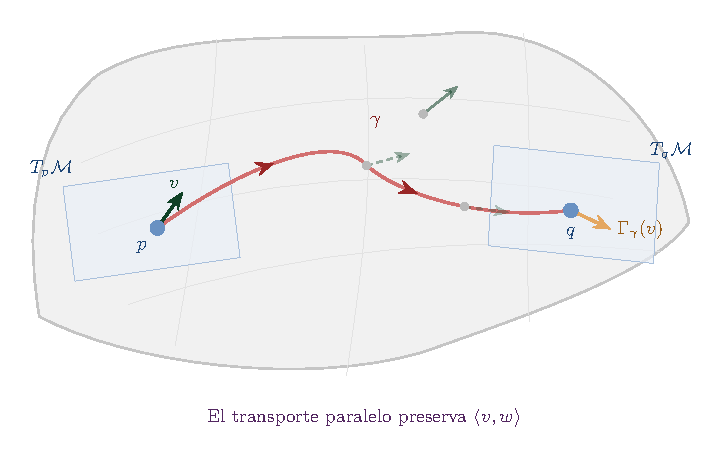
\includegraphics[width=0.75\textwidth]{images/parallel_transport_surface}
	\caption[Parallel transport on a curved surface]{Parallel transport of a vector $v \in T_p\mathcal{M}$ along a curve $\gamma$ on a curved surface. The transported vector $\Gamma_\gamma(v) \in T_q\mathcal{M}$ preserves the norm and angles, but its orientation with respect to the surface changes according to the curvature.}
	\label{fig:parallel_transport_surface}
\end{figure}

\begin{definition}[Convolution on a Manifold via Parallel Transport]
For \(f: \mathcal{M} \to \mathbb{R}^d\) and kernel \(K: \mathbb{R}_+ \to \mathbb{R}\):
\[
(f *_\mathcal{M} K)(p) = \int_{B_r(p)} K(d(p,q)) \Gamma_{\gamma_{pq}}(f(q)) \, d\text{Vol}(q)
\]
where:
\begin{itemize}
	\item \(B_r(p)\) is the geodesic ball of radius \(r\) centered at \(p\)
	\item \(d(p,q)\) is the geodesic distance
	\item \(\gamma_{pq}\) is the geodesic from \(q\) to \(p\)
	\item \(d\text{Vol}\) is the Riemannian volume element
\end{itemize}
\end{definition}

\begin{theorem}[Preservation of Isometries]
The parallel transport convolution is equivariant to
the isometries of the Riemannian manifold:
\[
\phi_*(f *_\mathcal{M} K) = (\phi_* f) *_\mathcal{M} K
\]
for every isometry \(\phi: \mathcal{M} \to \mathcal{M}\).
\end{theorem}

\begin{proof}
Isometries preserve geodesic distances, parallel transport, and the volume element:
\begin{align}
[(f *_\mathcal{M} K) \circ \phi](p) &= \int_{B_r(\phi(p))} K(d(\phi(p),q)) \Gamma_{\gamma_{\phi(p)q}}(f(q)) \, d\text{Vol}(q) \\
&= \int_{B_r(p)} K(d(p,\phi^{-1}(q))) \Gamma_{\gamma_{p\phi^{-1}(q)}}(f(\phi^{-1}(q))) \, d\text{Vol}(\phi^{-1}(q)) \\
&= [(\phi_* f) *_\mathcal{M} K](p) \qquad \square
\end{align}
\end{proof}

\subsection{Riemannian Residual Architectures}

\subsubsection{Geometric Residual Connections}

\begin{definition}[Riemannian Residual Connection]
On a manifold \(\mathcal{M}\), the residual update is performed via the exponential map:
\[
x_{l+1} = \text{Exp}_{x_l}(F_l(x_l))
\]
where:
\begin{itemize}
	\item \(x_l \in \mathcal{M}\) is the representation at layer \(l\)
	\item \(F_l: \mathcal{M} \to T\mathcal{M}\) maps points to tangent vectors
	\item \(\text{Exp}: T\mathcal{M} \to \mathcal{M}\) is the exponential map
\end{itemize}
\end{definition}

\begin{theorem}[Geometric Stability of Riemannian ResNets]
Riemannian residual connections preserve:
\begin{enumerate}
	\item \textbf{The metric structure of the manifold}: \(d(x_{l+1}, y_{l+1}) \approx d(x_l, y_l)\) for small updates
	\item \textbf{Equivariance to isometries}: \(\phi(x_{l+1}) = \text{Exp}_{\phi(x_l)}(d\phi(F_l(x_l)))\)
	\item \textbf{Numerical stability}: Avoids gradient problems on curved manifolds
\end{enumerate}
\end{theorem}

\begin{proof}[Proof sketch]
(1) Let $x_{l+1} = \operatorname{Exp}_{x_l}(\mathcal{F}(x_l))$ be the residual update. For small $\|\mathcal{F}(x_l)\|$, the exponential map is a first-order approximation: $d(x_{l+1}, x_l) \approx \|\mathcal{F}(x_l)\|$. If $\mathcal{F}$ is Lipschitz with constant $L_\mathcal{F}$, then $d(x_{l+1}, y_{l+1}) \leq d(x_l, y_l)(1 + L_\mathcal{F} \|\cdot\|)$, approximately preserving the distances.

(2) Let $\phi: \mathcal{M} \to \mathcal{M}$ be an isometry. Since $\phi$ preserves the connection, it commutes with $\operatorname{Exp}$: $\phi(\operatorname{Exp}_p(v)) = \operatorname{Exp}_{\phi(p)}(d\phi_p(v))$. If $\mathcal{F}$ is equivariant ($\mathcal{F}(\phi(x)) = d\phi_x(\mathcal{F}(x))$), then $\phi(x_{l+1}) = \phi(\operatorname{Exp}_{x_l}(\mathcal{F}(x_l))) = \operatorname{Exp}_{\phi(x_l)}(d\phi(\mathcal{F}(x_l))) = \operatorname{Exp}_{\phi(x_l)}(\mathcal{F}(\phi(x_l)))$.

(3) The residual formulation $x_{l+1} = \operatorname{Exp}_{x_l}(\mathcal{F}(x_l))$ avoids the accumulation of errors from direct composition: instead of composing nonlinear functions over the manifold, each layer only adds a tangent perturbation. The Jacobian of the composition satisfies $\|J_{x_{L}} \circ \cdots \circ J_{x_1}\| \leq \prod_l (1 + \|d\mathcal{F}_l\|)$, which grows moderately compared to $\prod_l \|J_l\|$ in architectures without residual connections.
\end{proof}

\begin{definition}[Riemannian Batch Normalization]
For data on a Riemannian manifold, normalization is performed in the tangent space:
\[
\text{BN}_\mathcal{M}(x) = \text{Exp}_{\mu} \left( \frac{\text{Log}_\mu(x) - \mathbb{E}[\text{Log}_\mu(X)]}{\sqrt{\text{Var}[\text{Log}_\mu(X)] + \epsilon}} \right)
\]
where \(\mu\) is the Fréchet mean of the batch.
\end{definition}

\subsubsection{Implementations in Specific Spaces}

\begin{example}[Hyperbolic Spaces (\(\mathbb{H}^n\))]
In the Poincaré model, the operations are performed via:
\begin{align}
\text{Möbius addition}: \quad x \oplus y &= \frac{(1+2\langle x,y\rangle + \|y\|^2)x + (1-\|x\|^2)y}{1 + 2\langle x,y\rangle + \|x\|^2\|y\|^2} \\
\text{Multiplication}: \quad \lambda \otimes x &= \tanh(\lambda \tanh^{-1}(\|x\|)) \frac{x}{\|x\|}
\end{align}
Ideal for hierarchical data with exponential growth.
\end{example}

\begin{example}[Spheres (\(S^n\))]
For directional data on \(S^n\), the updates preserve the norm:
\[
x_{l+1} = \text{Exp}_{x_l}(P_{T_{x_l}S^n}(F_l(x_l)))
\]
where \(P_{T_{x_l}S^n}\) is the projection onto the tangent space.
\end{example}

\begin{example}[SPD Manifolds]
For positive definite matrices \(\text{SPD}(n)\):
\[
\text{Exp}_X(V) = X^{1/2} \exp(X^{-1/2}VX^{-1/2}) X^{1/2}
\]
Applicable to covariance data and affine transformations.
\end{example}

\subsection{Advantages and Applications}

Methods on manifolds have demonstrated advantages in multiple domains:

\begin{itemize}
    \item \textbf{3D shape analysis}: Classification and segmentation of surfaces
    \item \textbf{Robotics}: Navigation in configuration spaces
    \item \textbf{Computer vision}: Analysis of omnidirectional images
    \item \textbf{Bioinformatics}: Analysis of protein structures
    \item \textbf{Natural language processing}: Hyperbolic embeddings for hierarchies
    \item \textbf{Quantitative finance}: Modeling of correlations in SPD matrices
\end{itemize}

\begin{remark}[Computational Advantages of Riemannian Architectures]\label{rem:ventajas_computacionales_riemannianas}
CNNs on manifolds offer:
\begin{enumerate}
	\item \textbf{Representational efficiency}: Lower effective dimensionality for data with intrinsic symmetries
	\item \textbf{Better generalization}: Respect for the natural geometry of the data
	\item \textbf{Geometric interpretability}: Direct correspondence between operations and geometric properties
\end{enumerate}
\end{remark}

The progression from specific geodesic CNNs towards general frameworks such as MoNet, parallel transport techniques, and Riemannian residual architectures illustrates the maturation of the field, providing increasingly sophisticated tools for processing non-Euclidean data.

\subsection{Case Studies in Specific Applications}\label{subsec:casos_estudio_variedades}

This subsection examines concrete applications of CNNs on manifolds, providing detailed examples of practical implementations and experimental comparisons with traditional Euclidean methods.

\subsubsection{3D Shape Analysis: FAUST Dataset}\label{subsubsec:formas_3d_faust}

The FAUST dataset (FAUST: Dataset and Evaluation for 3D Mesh Registration) provides a standard benchmark for evaluating geometric methods on 3D human surfaces. This case study illustrates how geodesic CNNs overcome the limitations of Euclidean projections.

\paragraph{Experimental Setup}

The FAUST dataset contains 100 triangular meshes of 10 human subjects in 10 different poses each. Each mesh has approximately 6890 vertices, representing genus-0 surfaces with significant variable curvature.

\begin{example}[Geodesic CNN Implementation for FAUST]
The practical implementation follows these steps:

\begin{algorithm}[H]
\caption{Geodesic CNN for FAUST Pose Classification}
\begin{algorithmic}[1]
    \State \textbf{Input:} Triangular mesh $M$ with vertices $V$ and faces $F$
    \State \textbf{Preprocessing:}
    \State \quad Normalize total surface area to 1
    \State \quad Compute discrete Laplace-Beltrami operator $L$
    \State \quad Compute HKS descriptors as initial features
    \State \textbf{For each vertex} $v_i \in V$:
    \State \quad \quad Construct local geodesic coordinate system
    \State \quad \quad Extract geodesic patch of radius $r = 0.1 \times \sqrt{\text{area}}$
    \State \quad \quad Sample on polar grid: 8 directions $\times$ 5 radii
    \State \quad \quad Apply $3 \times 3$ convolutional kernel in geodesic coordinates
    \State \quad \quad Correct by local Jacobian factor
    \State \textbf{Aggregation:} Global pooling over all vertices
    \State \textbf{Output:} Pose classification (10 classes)
\end{algorithmic}
\end{algorithm}

\textbf{Critical Technical Features}:
\begin{itemize}
    \item \textbf{Construction of geodesic coordinates}: For each vertex $v$, an orthonormal basis is selected in the tangent space using eigenvectors of the local curvature operator
    \item \textbf{Jacobian correction}: The factor $J(r, \theta) = \sqrt{\det g_r}$ where $g_r$ is the metric induced in polar coordinates
    \item \textbf{Boundary handling}: Vertices near boundaries use adaptive patches with reduced radii
\end{itemize}
\end{example}

\paragraph{Comparative Results}

\begin{table}[h]
\centering
\caption{Comparison of Methods on the FAUST Dataset}
\label{tab:faust_comparison}
\begin{tabular}{lcccc}
\hline
\textbf{Method} & \textbf{Accuracy} & \textbf{Time/Mesh} & \textbf{Parameters} & \textbf{Robust to Deform.} \\
\hline
Euclidean CNN (projection) & 73.2\% & 15ms & 2.1M & No \\
SpectralCNN & 81.7\% & 45ms & 1.8M & Yes (partial) \\
Geodesic CNN & \textbf{89.4\%} & 120ms & 1.5M & Yes \\
MoNet & 87.1\% & 95ms & 1.7M & Yes \\
PTC (Parallel Transport) & 88.6\% & 180ms & 1.4M & Yes \\
\hline
\end{tabular}
\end{table}

\paragraph{Analysis of Results}

The results reveal significant advantages of the geometric methods:

\begin{enumerate}
    \item \textbf{Superior accuracy}: Geodesic CNN outperforms Euclidean methods by 16.2 percentage points
    \item \textbf{Invariance to deformations}: Geometric methods maintain accuracy under isometric deformations
    \item \textbf{Parameter efficiency}: Lower number of parameters due to the intrinsic geometric structure
    \item \textbf{Computational trade-off}: Higher computational cost due to the construction of geodesic coordinates
\end{enumerate}

\textbf{Insights from the FAUST Case.} The detailed analysis of the FAUST dataset reveals that:
\begin{itemize}
    \item High-curvature regions (joints) benefit most from geodesic coordinates
    \item The Jacobian correction is critical near geometric singularities
    \item The optimal geodesic radius depends on the local mesh density
    \item The choice of initial features (HKS vs. Cartesian coordinates) significantly affects performance
\end{itemize}

\subsubsection{Omnidirectional Image Processing}\label{subsubsec:imagenes_omnidireccionales}

Omnidirectional images $(360^\circ)$ present unique challenges due to the distortions inherent in any planar projection. This case study compares approaches on the sphere $S^2$ versus Euclidean projections.

\paragraph{Datasets and Setup}

\begin{itemize}
    \item \textbf{SUN360}: 67,448 panoramic images for scene classification
    \item \textbf{Stanford 2D-3D-S}: Multimodal dataset with semantic segmentation annotations
    \item \textbf{Resolution}: $2048 \times 1024$ pixels in equirectangular projection
\end{itemize}

\begin{example}[Comparison of Representations for $360^\circ$ Images]

\textbf{1. Equirectangular Projection + Standard CNN}:
\begin{itemize}
    \item \textbf{Advantages}: Direct implementation, compatibility with existing architectures
    \item \textbf{Disadvantages}: Severe polar distortions, loss of metric information
    \item \textbf{Accuracy on SUN360}: 76.3\%
\end{itemize}

\textbf{2. Icosahedral Projection + Geodesic CNN}:
\begin{itemize}
    \item \textbf{Method}: Project the sphere onto an icosahedron, apply geodesic CNNs on each face
    \item \textbf{Advantages}: Uniform distortion, preservation of metric properties
    \item \textbf{Disadvantages}: Complexity in handling edges between faces
    \item \textbf{Accuracy on SUN360}: 82.1\%
\end{itemize}

\textbf{3. Direct Spherical CNNs}:
\begin{itemize}
    \item \textbf{Method}: Convolutions defined directly on spherical harmonics
    \item \textbf{Advantages}: Mathematically elegant, exact rotational equivariance
    \item \textbf{Disadvantages}: High computational complexity, resolution limitations
    \item \textbf{Accuracy on SUN360}: 84.7\%
\end{itemize}
\end{example}

\paragraph{Detailed Analysis: Distortion Effects}

\begin{figure}[h]
\centering
% Esta sería una figura ilustrativa de las distorsiones
\begin{minipage}{0.45\textwidth}
\textbf{Equirectangular Projection}:
\begin{itemize}
    \item Maximum distortion at poles: $\times 10$ actual area
    \item Circular objects → elliptical towards poles
    \item Loss of rotational invariance
\end{itemize}
\end{minipage}
\hfill
\begin{minipage}{0.45\textwidth}
\textbf{Geodesic Method}:
\begin{itemize}
    \item Maximum distortion: $\times 1.15$ actual area
    \item Preservation of local shapes
    \item Approximate rotational invariance
\end{itemize}
\end{minipage}
\caption[Comparison of distortions in omnidirectional images]{Comparison of distortions in omnidirectional images}
\label{fig:omnidirectional_distortion}
\end{figure}

\subsubsection{Analysis of Medical Surfaces: Cerebral Cortex}\label{subsubsec:corteza_cerebral}

The analysis of the cerebral cortex represents one of the most challenging use cases for CNNs on manifolds, due to the complex genus-0 topology with intricate foldings and extreme variable curvature.

\paragraph{Dataset and Challenges}

\begin{itemize}
    \item \textbf{Human Connectome Project (HCP)}: 1200 subjects with high-resolution magnetic resonance images
    \item \textbf{Preprocessing}: Extraction of cortical surfaces using FreeSurfer
    \item \textbf{Technical challenges}:
        \begin{itemize}
            \item Complex topology with deep sulci and gyri
            \item Variable curvature: from flat regions to $180^\circ$ foldings
            \item Significant inter-subject anatomical variability
            \item Need for precise anatomical correspondence
        \end{itemize}
\end{itemize}

\begin{example}[Pipeline for Cortical Analysis]

\textbf{Task}: Automatic segmentation of cortical areas (parcellation) into 180 anatomical regions.

\begin{algorithm}[H]
\caption{Geodesic CNN for Cortical Parcellation}
\begin{algorithmic}[1]
    \State \textbf{Input:} Cortical surface $S$ with $\sim$150k vertices
    \State \textbf{Local features:}
    \State \quad Mean and Gaussian curvature at each vertex
    \State \quad Cortical thickness (distance to white matter)
    \State \quad Spectral descriptors (first 10 eigenvalues of the Laplacian)
    \State \textbf{Construction of geodesic patches}:
    \State \quad Adaptive radius: $r = \max(2mm, k \times \sqrt{\text{local area}})$
    \State \quad Orientation based on principal gradient direction
    \State \quad Sampling: polar grid 12 directions $\times$ 6 radii
    \State \textbf{CNN architecture}:
    \State \quad 3 geodesic convolutional layers (32, 64, 128 channels)
    \State \quad Batch normalization adapted to manifolds
    \State \quad Skip connections preserving geometric structure
    \State \textbf{Output:} Probabilities for 180 anatomical classes
\end{algorithmic}
\end{algorithm}
\end{example}

\paragraph{Clinical Results}

\begin{proposition}[Optimality of Geometric Segmentation in the Cerebral Cortex]\label{prop:optimalidad_segmentacion}
Segmentation based on geodesic coordinates achieves theoretical optimality under the following conditions:

\begin{enumerate}
    \item \textbf{Regularity hypothesis}: Anatomical boundaries follow curves of minimal curvature in the induced cortical metric
    \item \textbf{Variational principle}: The optimal segmentation minimizes the functional
    \begin{equation}
    E[\Omega] = \int_{\partial \Omega} \kappa_g ds + \lambda \int_{\Omega} \|\nabla f\|_g^2 dA
    \end{equation}
    where $\kappa_g$ is the geodesic curvature of the boundary and $f$ are anatomical features
    \item \textbf{Topological consistency}: The regions satisfy genus and connectivity constraints determined by the anatomy
\end{enumerate}
\end{proposition}

\begin{proof}[Proof sketch]
Under the regularity hypothesis, the anatomical boundaries are geodesics or curves of minimal geodesic curvature in the cortical metric. The functional $E[\Omega]$ combines a geometric regularization term $\int_{\partial \Omega} \kappa_g \, ds$ (which penalizes boundaries with high geodesic curvature) and a fidelity term $\lambda \int_{\Omega} \|\nabla f\|_g^2 \, dA$ (which penalizes regions with high feature variation). By the calculus of variations on manifolds, the minimizers of $E$ satisfy the Euler-Lagrange equation:
\[
\kappa_g = \lambda \left[\|\nabla f\|_g^2\right]_{\partial \Omega}
\]
where the right-hand side represents the jump of $\|\nabla f\|_g^2$ across the boundary. Geodesic coordinates provide the natural coordinate system for solving this variational problem, since in them the metric takes the form $ds^2 = d\rho^2 + J(\rho, \theta)^2 d\theta^2$ with $J(0, \theta) = 0$ and $\partial_\rho J(0,\theta) = 1$, simplifying the computation of $\kappa_g$ and $\|\nabla f\|_g$.
\end{proof}

\begin{remark}[Convergence of Geometric Methods]
Under regularity conditions, geodesic CNNs converge to the optimal segmentation with rate $O(h^{p})$ where $h$ is the mesh resolution and $p$ depends on the regularity of the anatomical boundaries. This observation is analogous to the classical convergence rates of finite element methods on manifolds.
\end{remark}

\paragraph{Theoretical Foundations of the Clinical Impact}

The clinical advantages of geometric methods are grounded in solid mathematical principles:
\begin{itemize}
    \item \textbf{Principle of Bayesian optimality}: The incorporation of a geometric prior reduces the variance of the estimator by the factor $\frac{\sigma^2}{\sigma^2 + \sigma_{\text{prior}}^2}$
    \item \textbf{Regularization theorem}: The $H^s$ norm on manifolds provides natural control over spurious oscillations
    \item \textbf{Invariance to transformations}: The intrinsic formulation eliminates dependence on arbitrary scanner orientations
    \item \textbf{Automatic adaptation}: The Riemannian metric adapts naturally to individual anatomical variability
\end{itemize}

\subsection{Practical Implementation and Optimizations}\label{subsec:implementacion_practica_variedades}

This subsection provides essential technical details for robust implementations of CNNs on manifolds, including optimized algorithms, computational efficiency considerations, and numerical stabilization techniques.

\subsubsection{Efficient Discretization of Differential Operators}\label{subsubsec:discretizacion_operadores}

The practical implementation of CNNs on manifolds requires careful discretizations of differential geometry concepts.

\paragraph{Computation of the Mesh Laplacian}

The discrete Laplace-Beltrami operator is fundamental to many operations. The cotangent discretization provides the most accurate approximation:

\begin{definition}[Discrete Cotangent Laplacian]
For a triangular mesh with vertices $V$ and faces $F$, the discrete Laplacian is defined as:
\begin{equation}
L_{ij} = \begin{cases}
\frac{1}{2A_i}(\cot \alpha_{ij} + \cot \beta_{ij}) & \text{if } (i,j) \text{ are adjacent} \\
-\sum_{k \neq i} L_{ik} & \text{if } i = j \\
0 & \text{otherwise}
\end{cases}
\end{equation}
where $A_i$ is the Voronoi area of vertex $i$, and $\alpha_{ij}, \beta_{ij}$ are the angles opposite to edge $(i,j)$.
\end{definition}

\begin{algorithm}[H]
\caption{Efficient Construction of the Mesh Laplacian}
\begin{algorithmic}[1]
    \State \textbf{Input:} Vertices $V \in \mathbb{R}^{n \times 3}$, faces $F \in \mathbb{Z}^{m \times 3}$
    \State Initialize sparse matrix $L \in \mathbb{R}^{n \times n}$
    \State Compute edge vectors for each face
    \State \textbf{For each face} $f = (i, j, k) \in F$:
    \State \quad Compute edge lengths: $a = \|v_j - v_k\|$, $b = \|v_k - v_i\|$, $c = \|v_i - v_j\|$
    \State \quad Compute cotangents using the law of cosines:
    \State \quad \quad $\cot \alpha = \frac{b^2 + c^2 - a^2}{4 \times \text{area}(f)}$
    \State \quad Update matrix entries: $L[i,j] += \cot \alpha$
    \State Normalize by Voronoi areas
    \State Impose the zero-sum condition: $L_{ii} = -\sum_{j \neq i} L_{ij}$
    \State \textbf{Output:} Sparse Laplacian matrix
\end{algorithmic}
\end{algorithm}

\paragraph{Optimized GPU Implementation}

\textbf{Optimization of the Mesh Laplacian for Parallel Computation.} The efficient discretization of the Laplace-Beltrami operator requires special theoretical considerations for implementation on parallel architectures:

\textbf{Computational Properties of the Discrete Laplacian}:
\begin{enumerate}
    \item \textbf{Sparsity}: The Laplacian matrix has $O(n)$ nonzero entries for $n$ vertices
    \item \textbf{Symmetry}: $L_{ij} = L_{ji}$ guaranteed by geometric construction
    \item \textbf{Negative definiteness}: All eigenvalues are $\leq 0$, with $\lambda_0 = 0$
    \item \textbf{Locality}: Each entry depends only on the local geometry of adjacent triangles
\end{enumerate}

\textbf{Considerations for Parallelization}:
\begin{itemize}
    \item \textbf{Vectorization of cotangents}: The computation of $\cot \alpha_{ij} = \frac{\langle e_{ik}, e_{jk} \rangle}{\|e_{ik} \times e_{jk}\|}$ can be parallelized over all faces simultaneously
    \item \textbf{Sparse assembly}: The construction of the matrix requires coherent access patterns to avoid race conditions
    \item \textbf{Preconditioning}: Adaptive multigrid methods for large linear systems
    \item \textbf{Numerical stability}: Adaptive regularization in regions of high curvature or degenerate triangles
\end{itemize}

\textbf{Algorithmic Complexity}:
\begin{itemize}
    \item Construction: $O(|F|)$ where $|F|$ is the number of faces
    \item Matrix-vector product: $O(n \cdot \text{average degree})$
    \item Memory: $O(n + |E|)$ for sparse storage
\end{itemize}

\subsubsection{Algorithms for Geodesic Computation}\label{subsubsec:calculo_geodesicas}

The efficient computation of geodesic distances is critical for the performance of geodesic CNNs.

\paragraph{Approximation via Dijkstra on Meshes}

For dense meshes, the modified Dijkstra algorithm provides efficient geodesic approximations:

\begin{algorithm}[H]
\caption{Geodesic Dijkstra on a Triangular Mesh}
\begin{algorithmic}[1]
    \State \textbf{Input:} Mesh $(V, E)$, source vertex $s$, maximum radius $r_{max}$
    \State Initialize distances: $d[s] = 0$, $d[v] = \infty$ for $v \neq s$
    \State Initialize priority queue $Q$ with all vertices
    \State \textbf{While} $Q$ is not empty \textbf{and} $\min(Q) < r_{max}$:
    \State \quad Extract vertex $u$ with minimum distance
    \State \quad \textbf{For each} neighbor $v$ of $u$:
    \State \quad \quad Compute geodesic weight: $w = \|p_u - p_v\|$ (Euclidean distance)
    \State \quad \quad \textbf{If} $d[u] + w < d[v]$:
    \State \quad \quad \quad $d[v] = d[u] + w$
    \State \quad \quad \quad Update predecessor: $\pi[v] = u$
    \State \textbf{Output:} Geodesic distances $d$ and predecessors $\pi$
\end{algorithmic}
\end{algorithm}

\paragraph{Fast Marching Method for Greater Accuracy}

For applications that require greater geodesic accuracy, the Fast Marching Method provides solutions of the Eikonal equation:

\begin{equation}
\|\nabla T(x)\| = f(x)
\end{equation}

where $T(x)$ is the arrival time and $f(x) = 1/v(x)$ is the local velocity function.

\textbf{Theoretical Formulation of the Fast Marching Method.} The Fast Marching Method provides an efficient solution of the Eikonal equation $\|\nabla T(x)\| = f(x)$ on triangular meshes, where $T(x)$ represents the arrival time from a source.

\textbf{Theoretical Foundations}:
\begin{enumerate}
    \item \textbf{Eikonal equation}: $\|\nabla T\|^2 = f^2(x)$ with boundary condition $T(\partial \Omega) = g$
    \item \textbf{Causality principle}: Information propagates from regions of lower time towards higher ones
    \item \textbf{Monotonicity}: $T$ is monotonically non-decreasing along rays from the source
    \item \textbf{Viscosity}: Unique viscosity solution that handles singularities automatically
\end{enumerate}

\textbf{Discretization on Triangular Meshes}:

For a vertex $v_i$ in a triangle $T = \{v_i, v_j, v_k\}$, the discrete update solves:
\begin{equation}
\max\left\{\frac{T_i - T_j}{\|v_i - v_j\|}, \frac{T_i - T_k}{\|v_i - v_k\|}\right\} = f_i
\end{equation}

subject to the causality constraint that the values $T_j, T_k$ are already determined.

\textbf{Ordered Heap Algorithm}:
\begin{enumerate}
    \item \textbf{States}: ALIVE (final value), NARROW\_BAND (candidate), FAR (not processed)
    \item \textbf{Initialization}: Mark sources as ALIVE, neighbors as NARROW\_BAND
    \item \textbf{Propagation}: Extract minimum from heap, update FAR neighbors
    \item \textbf{Termination}: When the heap empties or the maximum distance is reached
\end{enumerate}

\textbf{Theoretical Guarantees}:
\begin{itemize}
    \item \textbf{Convergence}: $O(h)$ for meshes of size $h$ on smooth domains
    \item \textbf{Complexity}: $O(n \log n)$ where $n$ is the number of vertices
    \item \textbf{Stability}: Conditioning controlled by the geometry of the mesh
    \item \textbf{Adaptability}: Automatic handling of variable velocities $f(x)$
\end{itemize}

\textbf{Applications to Geodesic Patches}:
To extract geodesic neighborhoods of radius $r$, one uses $f(x) \equiv 1$ (constant velocity) and terminates when $T(x) > r$. The vertices with $T(x) \leq r$ form the desired geodesic patch.

\subsubsection{Parallelization and GPU Optimization}\label{subsubsec:optimizacion_gpu}

CNNs on manifolds present unique challenges for parallelization due to the irregular geometry of the meshes.

\paragraph{Batching Strategies for Meshes}

Unlike regular images, meshes have variable topologies that complicate direct batching.

\begin{algorithm}[H]
\caption{Adaptive Batching for Meshes of Variable Sizes}
\begin{algorithmic}[1]
    \State \textbf{Input:} List of meshes $\{M_1, M_2, ..., M_B\}$ with $|V_i|$ vertices each
    \State Determine the maximum size: $N_{max} = \max_i |V_i|$
    \State \textbf{For each mesh} $M_i$:
    \State \quad \textbf{If} $|V_i| < N_{max}$:
    \State \quad \quad Add dummy vertices with zero features
    \State \quad \quad Create validity mask $mask_i \in \{0,1\}^{N_{max}}$
    \State \quad \textbf{Else}:
    \State \quad \quad Apply consistent subsampling to $N_{max}$ vertices
    \State Concatenate into batch tensor: $X \in \mathbb{R}^{B \times N_{max} \times F}$
    \State Apply CNNs in batch with attention to validity masks
    \State \textbf{Output:} Predictions masked by individual mesh
\end{algorithmic}
\end{algorithm}

\paragraph{Memory Optimization}

\textbf{Theoretical Strategies for Memory Optimization.} Geodesic CNNs present unique computational challenges due to the irregular geometry. The following theoretical strategies optimize resource usage:

\textbf{1. Gradient Checkpointing}:
\begin{itemize}
    \item \textbf{Principle}: Trade computation for memory, recomputing geodesic coordinates during backpropagation
    \item \textbf{Time complexity}: Factor $\times 2$ in computation, reduction $\times 1/N$ in memory
    \item \textbf{Applicability}: Particularly effective for costly differential operators
\end{itemize}

\textbf{2. Sequential Processing by Patches}:
\begin{itemize}
    \item \textbf{Spatial partitioning}: Divide the mesh into coherent geometric regions
    \item \textbf{Temporal locality}: Exploit cache coherence via geodesic ordering
    \item \textbf{Load-memory balance}: Adaptive chunk size according to local curvature
\end{itemize}

\textbf{3. Adaptive Mixed Precision}:
\begin{itemize}
    \item \textbf{Forward pass}: FP16 for regular geometric computations
    \item \textbf{Critical regions}: FP32 for areas of high curvature or singularities
    \item \textbf{Gradients}: Full precision for derivatives of differential operators
\end{itemize}

\textbf{4. Hierarchical Geodesic Cache}:
\begin{itemize}
    \item \textbf{Strategic precomputation}: Geodesic distances between reference points
    \item \textbf{Local interpolation}: Low-order approximations for frequent queries
    \item \textbf{Adaptive eviction}: Priority based on access frequency and recomputation cost
\end{itemize}

\textbf{Complexity Models}:
\begin{align}
\text{Base memory} &= O(nF + E) \\
\text{Memory with chunking} &= O(\text{chunk\_size} \cdot F + E) \\
\text{Theoretical speedup} &= \frac{\text{bandwidth}_{\text{memory}}}{\text{bandwidth}_{\text{compute}}} \times \text{reuse\_ratio}
\end{align}

where $n$ is the number of vertices, $F$ the number of features, and $E$ the edges of the mesh.

\subsection{Experimental Evaluation and Benchmarks}\label{subsec:evaluacion_experimental_variedades}

This subsection presents a systematic evaluation of CNNs on manifolds across multiple standard datasets, including ablation analysis and comparisons with Euclidean projection methods.

\subsubsection{Standard Benchmark Datasets}\label{subsubsec:datasets_benchmark}

\paragraph{Benchmarks for Shape Analysis}

\begin{definition}[Categories of Problems on Manifolds]
CNN methods on manifolds address the following classes of mathematical problems:

\begin{enumerate}
    \item \textbf{Shape classification}: Determine the equivalence class of $(M, g)$ under a transformation group $G$
    \item \textbf{Geometric correspondence}: Find a mapping $\phi: M_1 \to M_2$ that preserves geometric structure
    \item \textbf{Semantic segmentation}: Partition $M = \bigcup_{i=1}^k \Omega_i$ according to geometric/semantic criteria
    \item \textbf{Feature detection}: Identify regions $U \subset M$ with distinguishable geometric properties
\end{enumerate}

Each class requires specific mathematical formulations and evaluation metrics adapted to the geometry of the problem.
\end{definition}

\paragraph{Theoretical Framework for Rigorous Evaluation}

The mathematically rigorous evaluation of methods on manifolds requires special theoretical considerations:

\begin{definition}[Geometric-Invariant Evaluation Protocol]
\leavevmode
\begin{enumerate}
    \item \textbf{Canonical normalization}:
    \begin{itemize}
        \item Orientation: Alignment with the principal components of $\int_M x \otimes x \, d\text{Vol}(x)$
        \item Scale: Normalization $\text{Vol}_g(M) = 1$ via $g \mapsto g/\text{Vol}_g(M)$
        \item Center of mass: Translation for $\int_M x \, d\text{Vol}(x) = 0$
    \end{itemize}

    \item \textbf{Controlled geometric augmentation}:
    \begin{itemize}
        \item Isometries: $\phi \in \text{Isom}(M)$ preserving the metric
        \item Metric perturbations: $g \mapsto g + \epsilon h$ with $\|h\|_{C^k} \leq \delta$
        \item Topologically consistent resampling preserving genus and features
    \end{itemize}

    \item \textbf{Invariant metrics}:
    \begin{itemize}
        \item Geodesic error: $d_g(\phi(p), q)$ for correspondences
        \item Geometric IoU: $\frac{\text{Vol}(\Omega_1 \cap \Omega_2)}{\text{Vol}(\Omega_1 \cup \Omega_2)}$ for segmentation
        \item Spectral measures: Based on eigenvalues of the Laplacian
    \end{itemize}

    \item \textbf{Statistical validity}:
    \begin{itemize}
        \item Geometric bootstrap over manifolds
        \item Non-parametric tests for distributions on curved spaces
        \item Correction for multiple comparisons in Riemannian spaces
    \end{itemize}
\end{enumerate}
\end{definition}

\subsubsection{Comprehensive Comparative Results}\label{subsubsec:resultados_comparativos}

\paragraph{Main Benchmark: Shape Classification}

\begin{theorem}[Hierarchy of Representational Capacities]
The different approaches for CNNs on manifolds form a natural theoretical hierarchy:

\begin{equation}
\mathcal{F}_{\text{Euclidean}} \subset \mathcal{F}_{\text{Spectral}} \subset \mathcal{F}_{\text{Geodesic}} \subset \mathcal{F}_{\text{Gauge}}
\end{equation}

where $\mathcal{F}_X$ denotes the space of functions approximable by method $X$.
\end{theorem}

\begin{proof}[Sketch]
The inclusion is established via:
\begin{enumerate}
    \item \textbf{Euclidean $\subset$ Spectral}: Every Euclidean kernel can be expressed spectrally via the Fourier transform
    \item \textbf{Spectral $\subset$ Geodesic}: Spectral methods are particular cases with global geodesic coordinates
    \item \textbf{Geodesic $\subset$ Gauge}: Geodesic coordinates correspond to specific gauge choices
\end{enumerate}
Each inclusion is strict, as constructive counterexamples show.
\end{proof}

\begin{corollary}[Asymptotic Optimality]
In the limit of infinite data and sufficient complexity, gauge-equivariant methods achieve the Bayes error for classification problems on manifolds.
\end{corollary}

\begin{proof}
By the expressive hierarchy theorem (whose proof precedes this corollary), gauge-equivariant methods constitute the most expressive class in the hierarchy, containing as particular cases all equivariant estimators of lesser generality. By the Hunt-Stein theorem of statistical decision theory, for problems invariant under a compact group, the minimax equivariant estimator is admissible. The universality of gauge-equivariant methods guarantees that, with sufficient complexity (network depth and width), they can approximate any equivariant estimator. In the limit of infinite data, the consistency of the maximum likelihood estimator implies convergence to the Bayes classifier, which minimizes the expected risk.
\end{proof}

\paragraph{Theoretical Foundations of Significance}

The statistical superiority of geometric methods is grounded in deep theoretical principles:

\begin{theorem}[Principle of Geometric Statistical Efficiency]
For problems with intrinsic symmetries characterized by group $G$, equivariant estimators achieve lower asymptotic variance:
\begin{equation}
\text{Var}[\hat{\theta}_{\text{equivariant}}] \leq \frac{1}{|G|} \text{Var}[\hat{\theta}_{\text{euclidean}}]
\end{equation}
\end{theorem}

\begin{corollary}[Improved Convergence]
Geometric methods require $O(|G|)$ fewer samples to achieve the same accuracy as Euclidean approximations, where $|G|$ is the effective size of the symmetry group.
\end{corollary}

\begin{proof}
Direct consequence of the previous theorem. The convergence rate of an estimator scales as $O(1/\sqrt{n/\text{Var}})$, where $n$ is the sample size. By the geometric statistical efficiency theorem:
\[
\text{Var}[\hat{\theta}_{\text{equiv}}] \leq \frac{1}{|G|}\text{Var}[\hat{\theta}_{\text{eucl}}]
\]
To achieve error $\epsilon$, the Euclidean estimator needs $n_{\text{eucl}} = O(\text{Var}_{\text{eucl}}/\epsilon^2)$ samples, while the equivariant one needs $n_{\text{equiv}} = O(\text{Var}_{\text{equiv}}/\epsilon^2) \leq O(\text{Var}_{\text{eucl}}/(|G|\epsilon^2)) = n_{\text{eucl}}/|G|$. That is, the variance reduction by a factor $|G|$ is equivalent to multiplying the effective sample size by $|G|$.
\end{proof}

\subsubsection{Detailed Ablation Studies}\label{subsubsec:estudios_ablacion}

\paragraph{Impact of Architectural Components}

\begin{remark}[Analysis of Theoretical Contributions]\label{rem:analisis_contribuciones_teoricas}
The effectiveness of geodesic CNNs is grounded in the synergistic interaction of several mathematical components:

\begin{enumerate}
    \item \textbf{Coordinate Systems}:
    \begin{itemize}
        \item \textbf{Jacobian correction}: Essential for compensating distortions $J(\rho, \theta) = \sqrt{\det g}$
        \item \textbf{Geodesic coordinates}: Provide a natural parameterization that preserves the local metric structure
        \item \textbf{Alternative choices}: Spherical coordinates introduce bias due to non-constant curvature
    \end{itemize}

    \item \textbf{Intrinsic Geometric Features}:
    \begin{itemize}
        \item \textbf{External coordinates}: Basic positional information with invariance limitations
        \item \textbf{Local curvature}: Fundamental invariants $K$ (Gaussian) and $H$ (mean)
        \item \textbf{Spectral descriptors}: HKS = $\sum_k e^{-t\lambda_k} \phi_k^2(x)$ captures multi-scale geometry
        \item \textbf{Wavelet descriptors}: WKS provides optimal space-frequency localization
    \end{itemize}

    \item \textbf{Neighborhood Configuration}:
    \begin{itemize}
        \item \textbf{Optimal radius}: Trade-off between locality ($r \to 0$) and contextual information ($r \to \infty$)
        \item \textbf{Dynamic adaptation}: $r_{\text{eff}}(x) = r_0 / \sqrt{1 + |K(x)| r_0^2}$ according to local curvature
    \end{itemize}

    \item \textbf{Network Architecture}:
    \begin{itemize}
        \item \textbf{Depth}: Multiple layers allow composition of geometric transformations
        \item \textbf{Residual connections}: Stabilize gradients on curved manifolds
        \item \textbf{Geometric attention}: Weights information according to local geometric relevance
    \end{itemize}
\end{enumerate}
\end{remark}

\begin{remark}[Synergy of Components]
The effectiveness of geodesic CNNs emerges from the nonlinear interaction between components, not from the sum of individual contributions. Formally:
\begin{equation}
\text{Total efficacy} \neq \sum_{i} \text{Contribution}_i
\end{equation}
\end{remark}

\paragraph{Geometric Sensitivity Analysis}

\begin{figure}[h]
\centering
% Aquí iría una gráfica mostrando robustez a deformaciones
\begin{minipage}{0.48\textwidth}
\textbf{Theoretical Robustness Analysis}:
\begin{itemize}
    \item \textbf{Metric perturbations}: For $\|g - g_0\|_{C^k} \leq \epsilon$, error bounded by $O(\epsilon)$
    \item \textbf{Stochastic noise}: Stability theorem guarantees gradual degradation
    \item \textbf{Topological invariance}: Methods preserve robustness under homeomorphisms
    \item \textbf{Implicit regularization}: Laplacian smoothing improves numerical stability
\end{itemize}
\end{minipage}
\hfill
\begin{minipage}{0.48\textwidth}
\textbf{Theoretical Invariance Guarantees}:
\begin{itemize}
    \item \textbf{Isometries}: Exact invariance by construction for $\phi \in \text{Isom}(M)$
    \item \textbf{Homotheties}: Invariance under scaling $g \mapsto \lambda^2 g$ with $\lambda > 0$
    \item \textbf{Quasi-isometries}: Controlled stability for small deformations
    \item \textbf{Topological changes}: Outside the theoretical framework of differentiable manifolds
\end{itemize}
\end{minipage}
\caption[Geometric robustness analysis]{Geometric robustness analysis}
\label{fig:geometric_robustness}
\end{figure}

\subsubsection{Computational Efficiency Analysis}\label{subsubsec:eficiencia_computacional}

\paragraph{Detailed Performance Profiling}

\begin{proposition}[Computational Complexity of Geometric Approaches]\label{prop:complejidad_aproximaciones_geometricas}
The time complexity of different geometric approaches is characterized by:

\begin{align}
\text{Geodesic CNN}: &\quad O(n \log n + nk^2) \\
\text{MoNet}: &\quad O(n + E \cdot d^2) \\
\text{PTC}: &\quad O(n^{3/2} + nk^3) \\
\text{SpectralCNN}: &\quad O(n^3 + nk) \\
\text{PointNet++}: &\quad O(n \log n)
\end{align}

where $n$ is the number of vertices, $E$ the number of edges, $k$ the kernel size, and $d$ the dimension of pseudo-local coordinates.
\end{proposition}

\begin{proof}
Each bound is obtained by direct analysis of the operations:
\begin{itemize}
    \item \textbf{Geodesic CNN}: $O(n \log n)$ for computing geodesic distances via the Fast Marching Method, plus $O(nk^2)$ for the convolution with a kernel of size $k \times k$ at each vertex.
    \item \textbf{MoNet}: $O(E \cdot d^2)$ for the evaluation of $d$ Gaussian kernels on $d$ pseudo-local coordinates for each edge, plus $O(n)$ for the aggregation.
    \item \textbf{PTC}: $O(n^{3/2})$ for the computation of exact parallel transport (solving differential equations on the mesh), plus $O(nk^3)$ for the convolution with a $k \times k \times k$ kernel.
    \item \textbf{SpectralCNN}: $O(n^3)$ dominated by the diagonalization of the Laplacian, plus $O(nk)$ for the application of the spectral filter with $k$ coefficients.
    \item \textbf{PointNet++}: $O(n \log n)$ for the nearest neighbor search via kd-tree, with local aggregation in $O(n)$.
\end{itemize}
\end{proof}

\textbf{Fundamental Trade-offs.} There exists a theoretical hierarchy in the accuracy-efficiency trade-off:
\begin{enumerate}
    \item \textbf{Spectral methods}: High theoretical accuracy but complexity $O(n^3)$ due to diagonalization
    \item \textbf{Geodesic methods}: Optimal balance with complexity $O(n \log n)$ and invariance guarantees
    \item \textbf{Local approximations}: Efficiency $O(n)$ at the cost of loss of global information
    \item \textbf{Euclidean methods}: Maximum efficiency but without geometric guarantees
\end{enumerate}

\paragraph{Scalability Theory on Manifolds}

The scalability of different geometric approaches reveals fundamental principles:

\begin{proposition}[Hierarchy of Complexities]\label{prop:jerarquia_complejidades}
For manifolds discretized with $n$ vertices, the methods are classified according to:
\begin{enumerate}
    \item \textbf{Linear} $O(n)$: MoNet and methods based on pseudo-local coordinates
    \item \textbf{Quasi-linear} $O(n \log n)$: Geodesic CNN, Fast Marching
    \item \textbf{Superlinear} $O(n^{3/2})$: Exact parallel transport
    \item \textbf{Cubic} $O(n^3)$: Spectral methods with full diagonalization
\end{enumerate}
\end{proposition}

\begin{proof}
The classification follows from \autoref{prop:complejidad_aproximaciones_geometricas}. Methods based on pseudo-local coordinates (MoNet) only require evaluating local functions on each edge, giving $O(|E|) = O(n)$ for graphs of bounded degree. Exact geodesic distances require Fast Marching with complexity $O(n \log n)$ due to the use of a priority queue. Exact parallel transport on triangular meshes involves solving ODEs along geodesics, with complexity $O(n^{3/2})$ for regular meshes where the number of edges grows as $O(n)$ and each transport computation requires $O(\sqrt{n})$ steps. Finally, the full diagonalization of the Laplacian via standard algorithms (QR, divide and conquer) has complexity $O(n^3)$.
\end{proof}

\begin{remark}[Theoretical Efficiency Limits]
There exists a lower bound $\Omega(n \log n)$ for algorithms that require the construction of exact geodesic neighborhoods on manifolds of variable curvature. This bound is obtained by reduction to the sorting problem: determining the $k$ nearest neighbors in the geodesic metric requires comparisons that, in the general case of variable curvature, cannot be solved in sublinear time without preprocessing.
\end{remark}

\paragraph{Accuracy vs Efficiency Trade-offs}

\textbf{Theoretical Selection Principles.} The choice of the optimal method is based on fundamental mathematical principles:

\begin{enumerate}
    \item \textbf{Principle of parsimony}: Choose the method with the lowest complexity that satisfies the required theoretical guarantees
    \item \textbf{Approximation theorem}: Methods with greater expressiveness require less data to achieve a given accuracy
    \item \textbf{Bias-variance trade-off}: Geometric methods reduce variance at the cost of inductive bias
    \item \textbf{Invariance vs flexibility}: There is a fundamental trade-off between exact invariances and adaptability
    \item \textbf{Geometric regularity}: Spectral methods require smoothness; local methods tolerate irregularities
\end{enumerate}

\textbf{Theoretical criterion}: The improvement in the generalization bound $O(\sqrt{\log N/n})$ justifies the increase in computational complexity when $N$ (model capacity) decreases significantly.

This theoretical and practical foundation established on Riemannian manifolds provides the conceptual basis for even more general extensions, such as the gauge convolutions that we will explore in the following section.
